\documentclass[letterpaper,12pt,oneside]{article}
\usepackage[top=1in, left=1.25in, right=1.25in, bottom=1in]{geometry}

\usepackage[T1]{fontenc}
\usepackage[utf8]{inputenc}
\usepackage[english]{babel}
\usepackage{caption, subcaption}
\usepackage{graphicx}
\usepackage{array}
\usepackage{booktabs}
\usepackage{amsmath,amssymb}
\usepackage{tikz}
\usetikzlibrary{automata, positioning, arrows.meta, bending}
\usepackage{imakeidx}
\usepackage{hyperref}
\usepackage{biblatex}
\addbibresource{bib/protocolo.bib}

\graphicspath{{./}{./figs/}}
\usepackage{setspace}

\hypersetup{
    colorlinks=true,
    linkcolor=black,
    citecolor=blue!70!black,
    urlcolor=blue!70!black
}

\begin{document}

% =========================================================================
% PORTADA INSTITUCIONAL
% =========================================================================
\begin{titlepage}
    \setlength{\parindent}{0pt} \setlength{\parskip}{0pt}

    \begin{center}
        \vfill 
        
        \begin{minipage}{\textwidth}
            \begin{center}
                
\includegraphics[width=4.2cm]{UNAM_LOGO2.png}    
            \end{center}     
            \begin{center}
                \Huge\textbf{Universidad Nacional Autónoma de México}
            \end{center} 
        \end{minipage}
            
        \vfill
        
        \begin{minipage}{0.85\textwidth}
            \begin{center}
                \Large Facultad de Ingeniería \\[0.2cm]
                \large Computer Engineering
            \end{center}
        \end{minipage}
        
        \begin{center}
            \vfill
            {\Large \textbf{Compilers (Group 5)}} \\[0.3cm]
            {\normalsize E.M. René Adrián Dávila Pérez}
        \end{center}
        
        \begin{center}
            \vspace*{0.8cm}
            {\LARGE \textbf{PROJECT REPORT: SYNTAX ANALYZER (PARSER) \& SYNTAX DIRECTED TRANSLATION (SDT)}}\\[0.3cm]
            {\large architecture package: \texttt{unam.fi.compilers.g5.05}}\\
            \vspace*{0.8cm}
            
            \begin{center}
                \textbf{Team members 05:} \\[0.25cm]
                319088058 \textit{(Documentation)} \\
                321634421 \textit{(Project Manager)} \\
                321037530 \textit{(Software developer)} \\
                424490412 \textit{(State Machine developer)} \\
                321009298 \textit{(Presenter)}
            \end{center}
            
            \bigskip
            
            \textbf{Group:} 5 \\
            \textbf{Semester:} 2027-1
        \end{center}
        
        \vfill
        
        \begin{center}
            {Ciudad Universitaria, CDMX. November 2026}\\
            {\footnotesize Repository: \url{https://github.com/alanvilchisssss/Compilers_Repository}}
        \end{center}
        \cleardoublepage
    \end{center}
\end{titlepage}

\tableofcontents
\clearpage

% =========================================================================
% SECTION 1: INTRODUCTION
% =========================================================================
\section{Introduction}

\subsection{Problem approach}
In this first phase of this project, we built a syntax analyzer, which is capable of reading code in the console of the program, or in a .txt file, which the programs reads, and based of the content classifies the lexemes in 5 different categories: reserved words, identifiers, operators, constants and punctuation signs. It's important to mention that our lexer only verifies that each word exists as an isolated form inside of the vocabulary that we defined previously in the project. Therefore, we don't validate the order, or structural order in which the words appear in the program or .txt file. 
In this second phase of our project, we are going to design an implement de Syntax Analyzer, and the Syntax-Directed Translation, which inside of the package code of unam.fi.compilers.g5.05, applying only the theoretical concepts seen in class, without any other automatic generator or libraries. The system revives the sequence of tokens generated by the lexer, builds a representation of the parsing three by using a predictive model known as Top Down LL(1), modeled on it's own state machine and afterwards verifies that the text actually follows the semantic rules of the SDT, distinguishing between syntactical errors, and semantic errors.


\subsection{Motivation}
The syntax analysis is a fundamental part in the theory of formal languages and the design of compilers because of: \cite{10.5555/576122}:
\begin{itemize}
    \item \textbf{Hierarchic validation:} A Context free grammar defines the hierarchy of sentences (as declarations and variables) allowing that a predictive parser verifies the grammar in an ideal time without extra process that might be inefficient for a huge load of data, even though, we aren't processing a huge quantity of data, it could mean time and memory for the program. 
    \item \textbf{Verifications depending on the context:} Because of a CFG on its own cant impose rules sensible to the context, like proving that a variable doesn't receive a value of another type which doesn't belong, or verifying previous declarations, implementing a SDT in the parsing three gives one mechanism to manage the attributes and validations in the .txt.
    \item \textbf{Precise mistake manager:} Distinguishing between structural mistakes of the grammar (\texttt{Parsing error...}) and the violations of the type or context of the program(\texttt{Parsing Success!}, followed by \texttt{SDT error...}) can give the user the right instructions in why is our program right or wrong.
\end{itemize}

\subsection{Objectives}
\textbf{General Objectives:} \\
The general objective of this part of the project is building a syntax analyzer as a Top-Down strategy, using a verifier of SDTs in out program \texttt{unam.fi.compilers.g5.05}, capable of validating sentences based of the tokens of the lexer, and using the different results of analyzing the semantic. 

\textbf{Specific Objectives:}
\begin{itemize}
    \item Adapting the output of the lexer analyzer so that we can manage the flow of the tokens so that the lexeme is conserved on it's own lexer category, line number and marker of the end of the input $\$ $.
    \item Modeling as a state machine and implementing a predictive parser descendant ($LL(1)$) based in the CFG, factorized by the left in the first release of the project. 
    \item Defining an implementing the semantic rules SDT through synthesized attributes and the heritage for the verification of the compatibility in types and declarations and initialization, (as \texttt{int x = 10;}), the calling format to \texttt{print} / \texttt{printf} and the register of a symbol table.
    \item Demonstrate theoretical and in the implementation the three scenarios required: Syntax and semantical verification, syntax success and semantical mistake, and syntactical mistakes. 
\end{itemize}

% =========================================================================
% SECTION 2: THEORETICAL FRAMEWORK
% =========================================================================
\section{Theoretical Framework}

\subsection{From Lexical Analysis to Predictive Top-Down Parsing}
According to the classic theory of compiler design~\cite{10.5555/576122}, the syntax analyzer receives a string of tokens coming from the lexical analyzer and checks if this string can be generated by the Context-Free Grammar (CFG) of the source language.

A \textbf{Top-Down Parser} builds the parse tree from the root (the start symbol) down to the leaves (the terminal tokens), trying to find a leftmost derivation for the input string. In particular, a \textbf{predictive $\mathbf{LL(1)}$ parser} scans the input from left to right (first $L$), produces a leftmost derivation (second $L$), and selects the exact production to apply by looking at only $1$ lookahead token without requiring backtracking.

\subsection{Left-Factored Context-Free Grammar (CFG)}
To guarantee a deterministic $LL(1)$ behavior without ambiguities caused by common prefixes, we use the left-factored Context-Free Grammar $G = (V, \Sigma, R, \text{Program})$, extended with the end-of-input marker $\$ $ and support for multiple statements:

\begin{align}
    \text{Program} &\to \text{StmtList} \ \$ \\
    \text{StmtList} &\to S \ \text{StmtList} \mid \varepsilon \\
    S &\to \text{Decl} \mid \text{Call} \\
    \text{Decl} &\to \text{type} \ \mathbf{id} \ \text{Decl'} \\
    \text{Decl'} &\to \mathbf{;} \;\Big|\; \mathbf{=} \ \text{Expr} \ \mathbf{;} \\
    \text{Call} &\to \text{print\_kw} \ \mathbf{(} \ \text{Expr} \ \text{Call'} \\
    \text{Call'} &\to \mathbf{)} \ \mathbf{;} \;\Big|\; \mathbf{,} \ \text{Arg} \ \mathbf{)} \ \mathbf{;}
\end{align}

where the lexical non-terminals derive into the terminal categories provided by the lexer:
\begin{align}
    \text{type} &\to \mathbf{int} \mid \mathbf{float} \mid \mathbf{char} \mid \mathbf{void} \\
    \text{print\_kw} &\to \mathbf{printf} \ \mid \ \mathbf{print} \\
    \text{Expr} &\to \mathbf{id} \mid \mathbf{constant} \\
    \text{Arg} &\to \mathbf{id} \mid \mathbf{constant}
\end{align}

By factoring the common prefixes ($\alpha_1 = \text{type} \ \mathbf{id}$ in declarations and $\alpha_2 = \text{print\_kw} \ \mathbf{(} \ \text{Expr}$ in print calls), the parser consumes the shared prefix first and uses the single lookahead token ($\mathbf{;}$ vs.\ $\mathbf{=}$ in $\text{Decl'}$, or $\mathbf{)}$ vs.\ $\mathbf{,}$ in $\text{Call'}$) to choose the valid production in a deterministic way.

\subsection{Syntax-Directed Translation (SDT) and Attributes}
A Context-Free Grammar on its own cannot verify context-sensitive rules, such as checking if the value assigned to a variable matches its declared type or if an identifier was already declared before~\cite{10.5555/576122}. To solve this, we use a \textbf{Syntax-Directed Definition (SDD)} implemented through a \textbf{Syntax-Directed Translation (SDT)} scheme.

An SDT scheme associates attributes with each node of the parse tree and evaluates semantic rules over the constructed tree:
\begin{itemize}
    \item \textbf{Synthesized attributes:} They are calculated in a parent node from the values of its child nodes (information goes up from the leaves to the root). For example, in the production $\text{Expr} \to \mathbf{constant}$, the node $\text{Expr}$ synthesizes its attribute $\text{Expr.type}$ by checking if the lexeme of the constant is an integer (\texttt{int}), a float (\texttt{float}), or a string (\texttt{string}).
    \item \textbf{Inherited attributes:} They are passed from a parent node or a left sibling to a child node (information goes down or moves sideways to the right). In the factored rule $\text{Decl} \to \text{type} \ \mathbf{id} \ \text{Decl'}$, the type declared in the left child ($\text{type.type}$) is passed as an inherited attribute ($\text{Decl'.inh\_type} = \text{type.type}$) to the sibling node $\text{Decl'}$ so that, when $\text{Decl'}$ evaluates an assignment ($\mathbf{=} \ \text{Expr} \ \mathbf{;}$), it knows which data type it must compare $\text{Expr.type}$ against.
\end{itemize}

\subsection{Formal Table of SDT Semantic Rules}
Table~\ref{tab:sdt_rules} shows the formal design of our Context-Free Grammar along with the SDT semantic actions associated with each production, where $\text{SymTab}$ represents the Symbol Table.

\begin{table}[htbp]
\centering
\caption{Productions of the Context-Free Grammar and associated SDT semantic rules.}
\label{tab:sdt_rules}
\begin{tabular}{lp{9cm}}
\toprule
\textbf{CFG Production} & \textbf{Semantic Rule / SDT Verification Action} \\
\midrule
$\text{Decl} \to \text{type} \ \mathbf{id} \ \text{Decl'}$ & 
1. Verify that $\text{type.type} \neq \texttt{void}$ and $\mathbf{id}.\text{lexeme} \notin \text{SymTab}$. \newline
2. Pass inherited attribute: $\text{Decl'.inh\_type} \leftarrow \text{type.type}$. \newline
3. If $\text{Decl'.ok} == \text{True}$, register $\text{SymTab}[\mathbf{id}.\text{lexeme}] \leftarrow \text{type.type}$; otherwise emit \texttt{SDT error...}. \\
\addlinespace
$\text{Decl'} \to \mathbf{;}$ & 
Simple declaration without initialization: $\text{Decl'.ok} \leftarrow \text{True}$. \\
\addlinespace
$\text{Decl'} \to \mathbf{=} \ \text{Expr} \ \mathbf{;}$ & 
Check type compatibility between the inherited and synthesized attributes: \newline
If $\text{Decl'.inh\_type} == \text{Expr.type}$, then $\text{Decl'.ok} \leftarrow \text{True}$; otherwise emit \texttt{SDT error...} on the current line. \\
\addlinespace
$\text{Call} \to \text{print\_kw} \ \mathbf{(} \ \text{Expr} \ \text{Call'}$ & 
Verify that the first argument of \texttt{print} or \texttt{printf} is a valid string literal: \newline
If $\text{Expr.type} == \texttt{string}$ and $\text{Call'.ok} == \text{True}$, it is valid; if not, emit \texttt{SDT error...}. \\
\addlinespace
$\text{Call'} \to \mathbf{)} \ \mathbf{;}$ & 
Simple call without extra arguments: $\text{Call'.ok} \leftarrow \text{True}$. \\
\addlinespace
$\text{Call'} \to \mathbf{,} \ \text{Arg} \ \mathbf{)} \ \mathbf{;}$ & 
If $\text{Arg.type} \neq \texttt{error}$, then $\text{Call'.ok} \leftarrow \text{True}$; if not, emit \texttt{SDT error...}. \\
\addlinespace
$\text{type} \to \mathbf{int} \mid \mathbf{float} \mid \mathbf{char} \mid \mathbf{void}$ & 
Synthesized attribute: $\text{type.type} \leftarrow \text{lexeme of the recognized type}$. \\
\addlinespace
$\text{Expr} \to \mathbf{constant}$ & 
Synthesized attribute $\text{Expr.type} \in \{\texttt{int}, \texttt{float}, \texttt{string}\}$ according to the format of the literal. \\
\addlinespace
$\text{Expr} \to \mathbf{id}$ & 
Search $\mathbf{id}.\text{lexeme}$ in $\text{SymTab}$. If it exists, $\text{Expr.type} \leftarrow \text{SymTab}[\mathbf{id}.\text{lexeme}]$; if it was not declared before, emit \texttt{SDT error...}. \\
\bottomrule
\end{tabular}
\end{table}

% =========================================================================
% SECTION 3: DEVELOPMENT
% =========================================================================
\section{Development}

Following the delivery instructions, the system was structured under the architecture package \texttt{unam.fi.compilers.g5.05} without depending on external tools for syntax generation.

\subsection{State Machine Design of the $LL(1)$ Parser}
To model the deterministic behavior of the syntax analyzer from the left-factored grammar, the finite state machine shown in Figure~\ref{fig:maquina_parser} was built using TikZ vector code.

\begin{figure}[htbp]
    \centering
    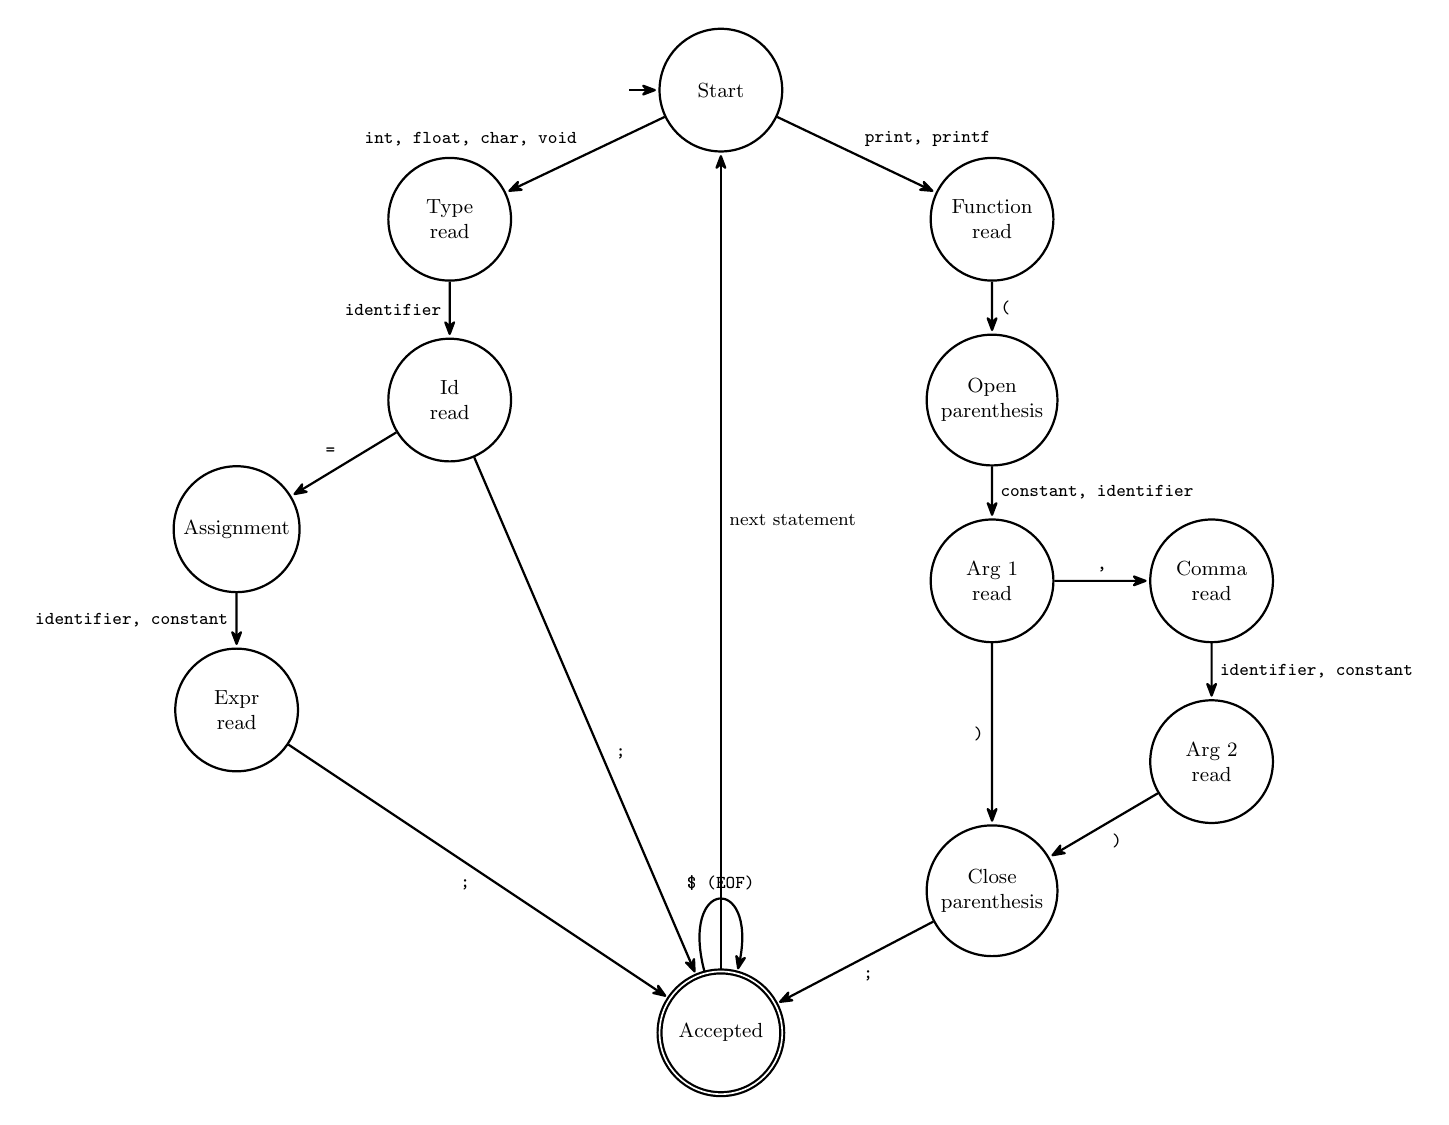
\begin{tikzpicture}[
        scale=0.82,
        transform shape,
        >={Stealth[round]},
        shorten >=1pt,
        auto,
        every state/.style={draw=black, thick, align=center, minimum size=1.9cm, font=\small},
        every edge/.style={draw=black, ->, >={Stealth[round]}, thick}
    ]
        % Nodo central de inicio
        \node[state, initial, initial text={}] (inicio) at (0,0) {Start};

        % Rama izquierda: Declaraciones
        \node[state] (tipo) at (-4.2, -2.0) {Type\\read};
        \node[state] (id) at (-4.2, -4.8) {Id\\read};
        \node[state] (asig) at (-7.5, -6.8) {Assignment};
        \node[state] (expr) at (-7.5, -9.6) {Expr\\read};

        % Rama derecha: Funciones print / printf
        \node[state] (func) at (4.2, -2.0) {Function\\read};
        \node[state] (par_ab) at (4.2, -4.8) {Open\\parenthesis};
        \node[state] (arg1) at (4.2, -7.6) {Arg 1\\read};
        \node[state] (coma) at (7.6, -7.6) {Comma\\read};
        \node[state] (arg2) at (7.6, -10.4) {Arg 2\\read};
        \node[state] (par_ci) at (4.2, -12.4) {Close\\parenthesis};

        % Nodo de aceptación
        \node[state, accepting] (aceptado) at (0, -14.6) {Accepted};

        % Transiciones Rama Izquierda
        \path
            (inicio) edge node[above left, font=\footnotesize] {\texttt{int, float, char, void}} (tipo)
            (tipo) edge node[left, font=\footnotesize] {\texttt{identifier}} (id)
            (id) edge node[above left, font=\footnotesize] {\texttt{=}} (asig)
            (asig) edge node[left, font=\footnotesize] {\texttt{identifier, constant}} (expr)
            (id) edge node[above right, pos=0.6, font=\footnotesize] {\texttt{;}} (aceptado)
            (expr) edge node[below left, font=\footnotesize] {\texttt{;}} (aceptado);

        % Transiciones Rama Derecha
        \path
            (inicio) edge node[above right, font=\footnotesize] {\texttt{print, printf}} (func)
            (func) edge node[right, font=\footnotesize] {\texttt{(}} (par_ab)
            (par_ab) edge node[right, font=\footnotesize] {\texttt{constant, identifier}} (arg1)
            (arg1) edge node[above, font=\footnotesize] {\texttt{,}} (coma)
            (coma) edge node[right, font=\footnotesize] {\texttt{identifier, constant}} (arg2)
            (arg1) edge node[left, font=\footnotesize] {\texttt{)}} (par_ci)
            (arg2) edge node[below right, font=\footnotesize] {\texttt{)}} (par_ci)
            (par_ci) edge node[below right, font=\footnotesize] {\texttt{;}} (aceptado);

        % Transiciones de retorno y EOF
        \path
            (aceptado) edge node[right, pos=0.55, font=\footnotesize] {next statement} (inicio)
            (aceptado) edge [loop above] node[font=\footnotesize] {\texttt{\$ (EOF)}} (aceptado);
    \end{tikzpicture}
    \caption{State machine of the predictive $LL(1)$ parser for the syntax analyzer.}
    \label{fig:maquina_parser}
\end{figure}

The automaton starts from the \textbf{Start} state and checks the lookahead token to branch without ambiguity into two main paths:
\begin{enumerate}
    \item \textbf{Left branch (Declarations --- $\text{Decl}$):} \\
    When receiving a type reserved word (\texttt{int}, \texttt{float}, \texttt{char}, \texttt{void}), it moves to the \textit{Type read} state, and after consuming an \texttt{identifier}, it advances to the \textit{Id read} state. At this exact point, the left factoring ($\text{Decl'}$) takes place:
    \begin{itemize}
        \item If the next token is the delimiter \texttt{;}, it goes directly to the final \textbf{Accepted} state (simple declaration).
        \item If the next token is the operator \texttt{=}, it moves to the \textit{Assignment} state, requires an \texttt{identifier} or \texttt{constant} to reach \textit{Expr read}, and finally consumes \texttt{;} to reach the \textbf{Accepted} state.
    \end{itemize}

    \item \textbf{Right branch (Output calls --- $\text{Call}$):} \\
    When reading \texttt{print} or \texttt{printf}, it advances to \textit{Function read}, requires the delimiter \texttt{(} towards \textit{Open parenthesis}, and consumes a \texttt{constant} or \texttt{identifier} to place itself in \textit{Arg 1 read}. In this state, the factoring of $\text{Call'}$ works as follows:
    \begin{itemize}
        \item If it receives \texttt{)}, it goes to \textit{Close parenthesis} and with \texttt{;} reaches the \textbf{Accepted} state.
        \item If it receives a comma (\texttt{,}), it moves to \textit{Comma read}, consumes the second argument (\textit{Arg 2 read}), closes with \texttt{)} towards \textit{Close parenthesis}, and finishes with \texttt{;} in \textbf{Accepted}.
    \end{itemize}
\end{enumerate}

From the \textbf{Accepted} state, if there are more tokens in the input flow, the automaton takes the \textit{next statement} transition back to \textbf{Start} (representing the recursion of $\text{StmtList}$), or it stays there and finishes successfully when finding the end-of-file marker \texttt{\$(EOF)}. Any token outside the described transitions causes an immediate rejection and outputs \texttt{Parsing error...} on the corresponding line.

\subsection{Functional Description of the Implementation}
Following the methodological guidelines, below we conceptually describe the functional architecture implemented in the four sequential modules of the system:

\begin{enumerate}
    \item \textbf{Input Acquisition Module (\texttt{cadena\_input}):} \\
    It keeps the dual interface that allows the user to enter a statement directly from the interactive terminal or read a source code file with a \texttt{.txt} extension using exception handling.

    \item \textbf{Lexical Analysis Module with Line Tracking (\texttt{ANALIZADOR\_LEXICO}):} \\
    It splits the input flow line by line and applies the master regular expression pattern that removes single-line and multi-line comments. Unlike the first phase, besides grouping lexemes by category, it builds an ordered sequential list of dictionaries where each token stores three attributes: its category (\texttt{tipo}), its original string (\texttt{lexema}), and its row number (\texttt{linea}), attaching the sentinel token \texttt{EOF} ($\$$) at the end.

    \item \textbf{Syntax Analysis Module (\texttt{PARSING}):} \\
    It directly implements in code the state machine from Figure~\ref{fig:maquina_parser} using a current position index and a helper consumption operation (\texttt{consumir}). It sequentially validates the factored productions $\text{Decl}$ and $\text{Call}$. If every transition is satisfied until reaching \texttt{EOF}, it builds the node structure of the parse tree (\texttt{arbol\_sintactico}) and outputs \texttt{Parsing Success!}; if an invalid transition happens, it stops the process and returns the exact line of the syntax error.

    \item \textbf{SDT Semantic Verification Module (\texttt{verificar\_sdt}):} \\
    It receives the parse tree generated by the parser and initializes a Symbol Table structure (\texttt{tabla\_simbolos}). It goes through each validated statement applying the rules from Table~\ref{tab:sdt_rules}: it checks that no variables are declared as \texttt{void}, that there are no duplicated identifiers or variables used without a previous declaration, that in every assignment the inherited attribute of the variable type matches the synthesized attribute of the expression (\texttt{obtener\_tipo\_constante}), and that the first argument of \texttt{print}/\texttt{printf} is strictly of type \texttt{string}.
\end{enumerate}

\subsection{Description of the Executed Tests}
According to the project specifications, three representative test scenarios were designed and theoretically justified:

\begin{enumerate}
    \item \textbf{Case 1 --- Valid Syntax and Verified SDT Semantics (\texttt{int x = 10;}):} \\
    \textbf{Theoretical argument:} The lexer produces the sequence $[\texttt{keyword(int)}, \texttt{identifier(x)}, \texttt{operator(=)}, \texttt{constant(10)}, \texttt{punctuation(;)}, \$]$. The $LL(1)$ parser follows the state machine path \textit{Start} $\to$ \textit{Type read} $\to$ \textit{Id read} $\to$ \textit{Assignment} $\to$ \textit{Expr read} $\to$ \textit{Accepted}, printing \texttt{Parsing Success!}. Afterwards, the SDT verifier propagates the inherited attribute $\text{Decl'.inh\_type} = \texttt{int}$ and compares it against the synthesized attribute $\text{Expr.type} = \texttt{int}$ deduced from the integer constant \texttt{10}. Since the equality $\texttt{int} == \texttt{int}$ is met and there is no previous declaration of \texttt{x} in the Symbol Table, the variable is registered and the system outputs \texttt{SDT Verified!}.

    \item \textbf{Case 2 --- Valid Syntax but SDT Semantic Error (\texttt{int x = "hello";}):} \\
    \textbf{Theoretical argument:} At a context-free level, both the number \texttt{10} and the string \texttt{"hello"} belong to the terminal category \texttt{constant}. Because of this, the sequence $[\texttt{keyword(int)}, \texttt{identifier(x)}, \texttt{operator(=)}, \texttt{constant("hello")}, \texttt{punctuation(;)}]$ satisfies all the transitions of the parser state machine and produces \texttt{Parsing Success!}. However, during the SDT semantic evaluation over the built tree, the inherited attribute requires an integer type ($\text{Decl'.inh\_type} = \texttt{int}$), while the literal in quotes synthesizes a string type ($\text{Expr.type} = \texttt{string}$). The compatibility rule $\texttt{int} == \texttt{string}$ is false, triggering \texttt{SDT error...} and reporting \texttt{error in line 1}.

    \item \textbf{Case 3 --- Direct Syntax Error (\texttt{int x = 10} without a semicolon):} \\
    \textbf{Theoretical argument:} When evaluating the assignment branch in the state machine, the parser consumes \texttt{=} and the constant \texttt{10}, reaching the \textit{Expr read} state, where the only valid transition towards \textit{Accepted} requires the terminal delimiter \texttt{;}. Instead, the analyzer finds the end-of-input marker $\$ $ (\texttt{EOF}). Since there is no transition for $\$ $ from \textit{Expr read}, the derivation is rejected before completing the tree and the system outputs \texttt{Parsing error...}. Given that the SDT scheme needs a valid parse tree to evaluate its attributes, the syntax failure prevents the semantic verification and consequently reports \texttt{SDT error...} and \texttt{error in line 1}.
\end{enumerate}

% =========================================================================
% SECTION 4: RESULTS
% =========================================================================
\section{Results}

Below we present the results obtained when running the system under the different evaluation cases.

\begin{figure}[htbp]
    \centering
    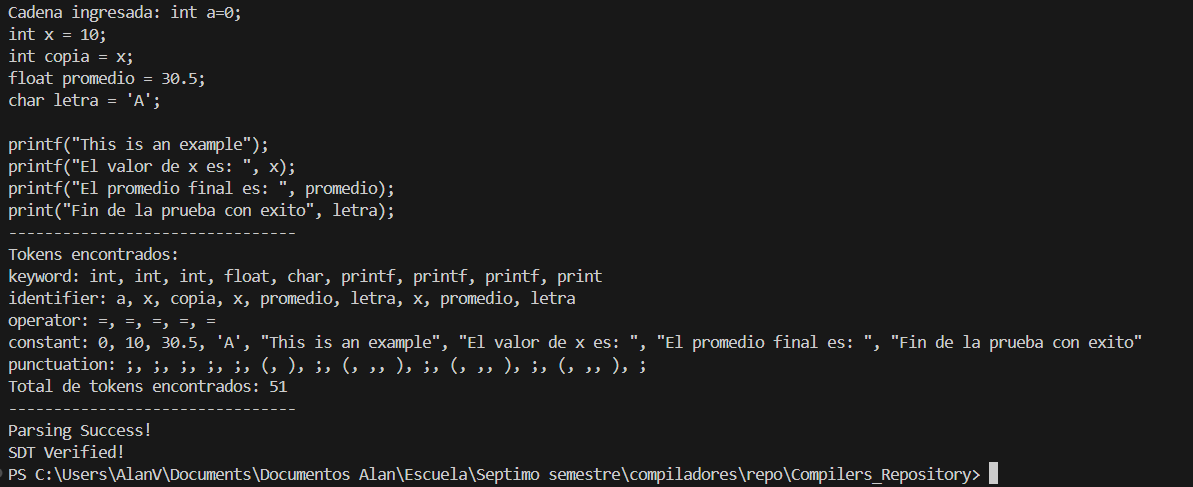
\includegraphics[width=0.85\textwidth]{caso1.png} 
    %\framebox[0.85\textwidth]{\rule{0pt}{3.2cm} \texttt{int x = 10;  -->  Parsing Success! / SDT Verified!}}
    \caption{Successful execution in both the $LL(1)$ syntax analysis and the SDT semantic verification for the statement \texttt{int x = 10;}.}
    \label{fig:res_caso1}
\end{figure}

%In Figure~\ref{fig:res_caso1}, we can see the complete validation of the model statement from the specification, confirming the recognition of the grammatical structure and the matching of integer types.

\begin{figure}[htbp]
    \centering
    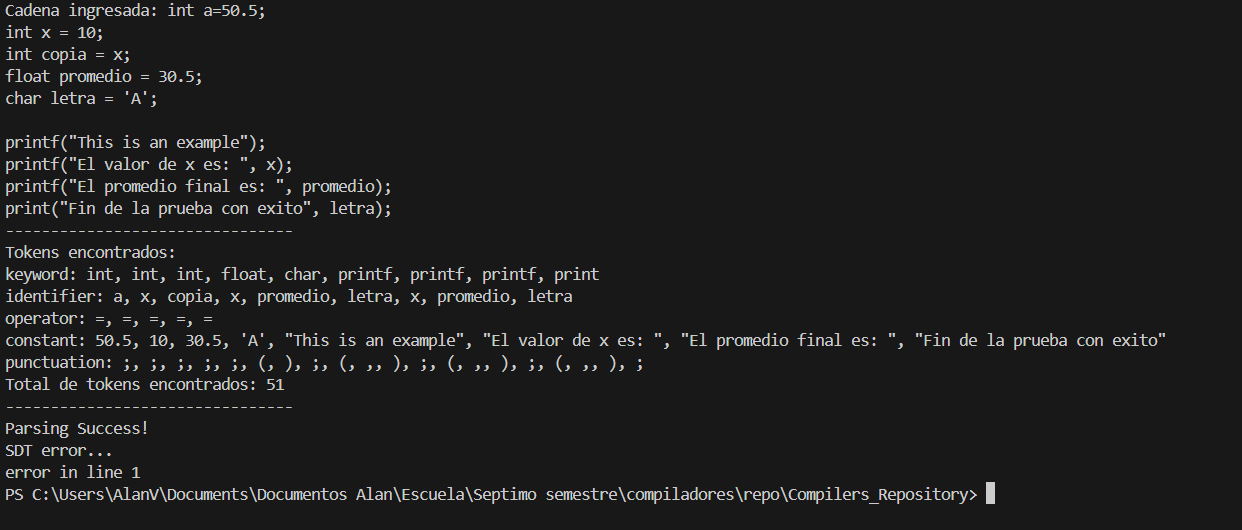
\includegraphics[width=0.85\textwidth]{caso2.png} 
    %\framebox[0.85\textwidth]{\rule{0pt}{3.2cm} \texttt{int x = "hello";  -->  Parsing Success! / SDT error... / error in line 1}}
    \caption{Execution with a valid syntactic structure but SDT semantic rejection due to type incompatibility.}
    \label{fig:res_caso2}
\end{figure}

%Figure~\ref{fig:res_caso2} experimentally shows the separation between context-free syntax and semantics: the parser approves the structure of the assignment, but the SDT verifier detects the conflict between the inherited type (\texttt{int}) and the synthesized type (\texttt{string}).

\begin{figure}[htbp]
    \centering
     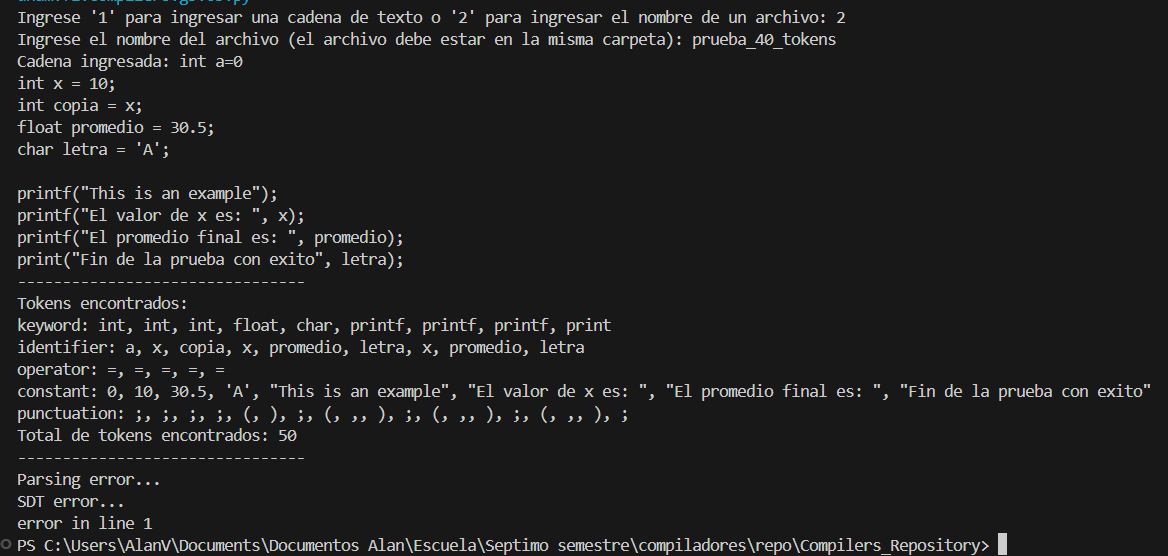
\includegraphics[width=0.85\textwidth]{caso3.png} 
    %\framebox[0.85\textwidth]{\rule{0pt}{3.2cm} \texttt{int x = 10  -->  Parsing error... / SDT error... / error in line 1}}
    \caption{Detection of a direct syntax error when omitting the end-of-statement delimiter.}
    \label{fig:res_caso3}
\end{figure}

%In Figure~\ref{fig:res_caso3}, we verify the immediate rejection of the parser when facing an incomplete statement, reporting the exact line of the problem. Finally, Table~\ref{tab:resumen_pruebas} summarizes the set of tests executed on the system.

\begin{table}[htbp]
\centering
\caption{Comparative summary of the cases evaluated in the Parser and SDT verifier.}
\label{tab:resumen_pruebas}
\begin{tabular}{lllp{5.8cm}}
\toprule
\textbf{Test Input} & \textbf{Parser Output} & \textbf{SDT Output} & \textbf{Technical Justification} \\
\midrule
\texttt{int x = 10;} & \texttt{Parsing Success!} & \texttt{SDT Verified!} & Satisfies the $\text{Decl}$ rule and attributes match ($\texttt{int} == \texttt{int}$). \\
\addlinespace
\texttt{printf("Example");} & \texttt{Parsing Success!} & \texttt{SDT Verified!} & Satisfies the factored $\text{Call}$ rule and the first argument is a \texttt{string}. \\
\addlinespace
\texttt{int x = "hello";} & \texttt{Parsing Success!} & \texttt{SDT error...} & Valid syntax, but SDT fails due to type mismatch ($\texttt{int} \neq \texttt{string}$). \\
\addlinespace
\texttt{int x = 30.5;} & \texttt{Parsing Success!} & \texttt{SDT error...} & Valid syntax, but SDT fails due to type incompatibility ($\texttt{int} \neq \texttt{float}$). \\
\addlinespace
\texttt{void a = 10;} & \texttt{Parsing Success!} & \texttt{SDT error...} & Grammatically \texttt{void} is a \texttt{type}, but SDT forbids \texttt{void} variables. \\
\addlinespace
\texttt{int x = 10} & \texttt{Parsing error...} & \texttt{SDT error...} & Missing the required terminal \texttt{;} at the end of the declaration. \\
\addlinespace
\texttt{int = 10;} & \texttt{Parsing error...} & \texttt{SDT error...} & Missing the required \texttt{identifier} token after the \texttt{int} type. \\
\bottomrule
\end{tabular}
\end{table}

% =========================================================================
% SECTION 5: CONCLUSIONS
% =========================================================================
\section{Conclusions}

The theoretical and experimental analysis of this second phase allows us to establish the following technical conclusions:

\begin{itemize}
    \item \textbf{Direct correspondence between Left Factoring and the $LL(1)$ State Machine:} The factoring applied in the first delivery allowed us to model the syntax analyzer through a deterministic automaton free of ambiguous transitions. By delaying the branching until the states \textit{Id read} (to choose between \texttt{;} and \texttt{=}) and \textit{Arg 1 read} (to choose between \texttt{)} and \texttt{,}), the parser works in linear time $O(n)$ by checking a single lookahead token without requiring backtracking.
    \item \textbf{Separation between context-free grammars and context-sensitive rules (SDT):} The modular architecture proved that syntactic validity is a necessary condition, but it is not enough to guarantee the coherence of a program. Cases like \texttt{int x = "hello";} prove that the parser only validates the structural sequence of lexical categories, while the SDT scheme has the responsibility of propagating inherited and synthesized attributes along with the Symbol Table to detect type mismatches.
    \item \textbf{Propagation of lexical metadata for accurate diagnosis:} Enriching the structure of each token from the lexical analyzer with its source line number and adding the end-of-file sentinel symbol ($\$$) was essential to synchronize the acceptance transitions of the automaton and output exact diagnostics under the \texttt{error in line n} standard.
\end{itemize}

\printbibliography

\end{document}